\documentclass[xcolor=svgnames]{beamer}

% #### graphics and schemes
\usepackage{graphicx}
\graphicspath{{img/}}
\usepackage{tikz}
\usetikzlibrary{shapes,decorations,mindmap,trees}
\usepackage[all]{xy} %needed for block diagrams
\usepackage{etex} % needed for block diagrams
\usepackage{array}
\usepackage{dirtree}
\usepackage{listings}
\usepackage{ccicons}

% #### theme
\useoutertheme{sidebar}
\useinnertheme{circles}
\usecolortheme{sidebartab}
\usecolortheme{seahorse}
\beamertemplatenavigationsymbolsempty

% #### colors
\usepackage{xcolor}
\definecolor{hughesblue}{rgb}{.9,.9,1} %A blue I like to use for highlighting, matches Hughes Hallet's book

% #### layouts
\usepackage{multicol}
\usepackage[labelfont=footnotesize,textfont=scriptsize,bf]{caption}
\usepackage{subfig}

% #### math
\usepackage[squaren]{SIunits}

% #### fonts
\usepackage[utf8]{inputenc}
\usepackage[italian]{babel}
\usepackage[T1]{fontenc}
\usepackage{cmbright}

% #### mainmatter
\title[Introduzione a GRASS in archeologia]{Introduzione all'utilizzo di GRASS GIS in archeologia: un manuale collaborativo}
\author[Francesco de Virgilio]{Francesco de Virgilio \\ \texttt{\tiny francesco.devirgilio@openoia.org}}
\institute[Università degli Studi di Bari]{
	%\inst{1}%
	O.I.A. --- Open Idea for Archaeology\\
	\emph{Università degli Studi di Bari}}
	% \and
	% \inst{2}%
	% School for Computational Science\\
	% Florida State University}

%% ##### logo matter ####
\pgfdeclaremask{uniba}{uniba-logo}
\pgfdeclareimage[mask=uniba,width=1.2cm]{uniba-logo}{img/oia-logo}
\logo{\vbox{\vskip0.1cm\hbox{\pgfuseimage{uniba-logo}}}}


\begin{document}

	% #### automatically prints toc when section starts
	\AtBeginSection[]
		{
		\begin{frame}
			\frametitle{Sommario}
			\begin{multicols}{2}
				\tableofcontents[currentsection]
			\end{multicols}
		\end{frame}
		}

	{
	\usebackgroundtemplate{
\includegraphics[width=1.2\paperwidth]{img/gnewarch}}
	\begin{frame}
		\titlepage
	\end{frame}
	}

	\section*{Sommario}

		\begin{frame}{Sommario}
			\begin{multicols}{2}
				\tableofcontents
			\end{multicols}
		\end{frame}
		
	\section{Perchè GRASS GIS}

		\begin{frame}{\textit{Background}}
			\begin{itemize}
				\item 2009, Cattedra di Archeologia Medievale, UniBa: necessità di gestire grandi quantità di dati archeologici georeferenziati
				\item hardware limitato, assenza di \textit{know-how}
				\item risorse economiche limitate, impossibile acquistare licenze software
			\end{itemize}
		\end{frame}

		% -----------------------------------------------------

		\begin{frame}{Perché GRASS}
			Pros:\\
			\begin{itemize}
				\item gestire enormi quantità di dati in maniera efficiente e precisa
				\item supporto a quasi tutti i formati e gli standard
				\item funzioni estese: circa 400 moduli disponibili
				\item licenza libera (GNU GPL): possibile distribuirlo gratuitamente agli studenti ed organizzare laboratori
				\item ottima documentazione in lingua inglese
				\item estendibilità e automazione (script)
			\end{itemize}
		\end{frame}

		% -----------------------------------------------------

		\begin{frame}{Perché GRASS}
			Cons:\\
			\begin{itemize}
				\item \alert{curva di apprendimento} ripida
				\item assenza di documentazione in lingua italiana orientata all'utilizzo in archeologia
				\item assenza di \alert{corpus ordinato} di procedure e metodi per l'archeologia
				\item difficoltà nell'approccio al terminale (spesso il più efficace)
			\end{itemize}
		\end{frame}

	\section{I GIS liberi in archeologia}

		\begin{frame}{Esperienze, standard e ricerca}
			\begin{beamerboxesrounded}{~}
				L'introduzione di GRASS e GFLOSS in ambito archeologico segna un passo avanti nella ricerca e nell'utilizzo di standard aperti in \emph{archeoinformatica}.
			\end{beamerboxesrounded}
		\end{frame}

		% -----------------------------------------------------

		\begin{frame}{Esperienze, standard e ricerca}
			L'utilizzo di GRASS nel settore archeologico:
			\begin{itemize}
				\item quasi-assenza di \alert{procedure standard}
				\item ricchezza di \alert{casi di studio}
				\item ogni nuova esperienza segna un caso di studio e la ricerca di nuove soluzioni;
				\item l'aumento delle esperienze descrive (involontariamente) una tendenza alla definizione di nuovi standard e procedure condivise
			\end{itemize}
		\end{frame}

		% -----------------------------------------------------

		\begin{frame}{Esperienze nel settore}
			\begin{itemize}
				\item Arc-Team s.n.c., \emph{voxel} (GRASS meeting 2006)
				\item Emanuel Demetrescu, archeologia urbana di Roma (2008)
				\item Michael Barton, archeologo/antropologo statunitense, è all'interno del team di sviluppo di GRASS
				\item Fronza, Nardini, Valenti, ``Informatica ed Archeologia Medievale''
			\end{itemize}
		\end{frame}

	\section{GRASS GIS nella didattica}

		\begin{frame}{Didattica del GFLOSS, un problema sociale}
			\begin{itemize}
				\item didattica universitaria ``concentrica'': partendo da una persona o un team di riferimento, le nuove esperienze circoscrivono le precedenti
				\item questo modello di sviluppo ha il suo punto di debolezza nella necessità di trovare un riferimento didattico
				\item esperienza di Bari: assenza di un riferimento
			\end{itemize}
		\end{frame}

		% -----------------------------------------------------

		\begin{frame}{Didattica del GFLOSS, un problema sociale}\label{sli:social}
			\begin{tikzpicture}[scale=0.8]
			  \path[mindmap,concept color=black,text=white]
			    node[concept] {GNewArchaeology}
			    [clockwise from=0]
			    child[concept color=green!50!black]
			    {
			      node[concept] {practical}
			      [clockwise from=90]
			      node[concept] {algorithms}
			      node[concept] {data structures}
			      node[concept] {pro\-gramming languages}
			      node[concept] {Bari}
			    }  
			    child[concept color=blue] {
			      node[concept] {Ferrara}
			      [clockwise from=-30]
			      child { node[concept] {Napoli} }
%			      child { node[concept] {WWW} }
			    }
			    child[concept color=red] { node[concept] {Padova} }
			    child[concept color=orange] { node[concept] {Trento} };
			\end{tikzpicture}
		\end{frame}

		% -----------------------------------------------------

		\begin{frame}{Smontare il sistema concentrico con una rete di conoscenze}
			\begin{itemize}
				\item creazione di un \alert{corpus didattico} esauriente e disponibile gratuitamente
				\item disponibilità al continuo mutamento, ampliamento e collaborazione
				\item posizionare sullo stesso piano le procedure e le rispettive applicazioni nei casi di studio
			\end{itemize}
		\end{frame}

		% -----------------------------------------------------

		\begin{frame}
			\newcommand*{\titleTH}{\begingroup% T&H Typography
			\raggedleft
			\definecolor{shadecolor}{gray}{0.75}
			\vspace*{\baselineskip}
			{\Large Francesco de Virgilio}\\[0.167\textheight]
			\hrule \vspace*{0.5cm}
			{\bfseries \large \fontsize{8mm}{10mm}\selectfont Introduzione all'utilizzo di}\\[\baselineskip]
			{\textcolor{red}{\huge \fontsize{15mm}{17mm}\selectfont GRASS GIS}}\\[\baselineskip]
			\makebox[0in][l] {\scalebox{1}[-1]{\textcolor{shadecolor}{{\normalsize\fontsize{8mm}{10mm}\selectfont{\textsl{in Archeologia}}}}}}{\textcolor{red}{\normalsize\fontsize{8mm}{10mm}\selectfont{\textsl{in Archeologia}}}}
			\vfill
%			{\large Università degli Studi di Bari}\par
%			\vspace{0.3cm}
%			{\small Corso di Laurea Triennale in\\Scienza e tecnologia per la Diagnostica e la Conservazione dei Beni Culturali}\par
%			\vspace*{3\baselineskip}
			\endgroup}
			\thispagestyle{empty}
			\titleTH
		\end{frame}

	\section{Impostazione editoriale}

		\begin{frame}{\emph{Key facts}}
			\begin{itemize}
				\item manuale orientato a studenti con basi di GIS
				\item equiparazione delle funzioni da terminale e da interfaccia (wxPython)
				\item appendice esteso sulle proiezioni cartografiche
			\end{itemize}
		\end{frame}

		% -----------------------------------------------------

		\begin{frame}{\emph{Key facts}}
		\framesubtitle{consultazione rapida: caselle con comandi di pronto utilizzo e consigli}
			\begin{center}
				\begin{tikzpicture}[thick,scale=0.006\textwidth] %this measure generates a page half the text size
					\draw[fill=black!5]
					(0pt,0pt) --
					(100pt,0pt) [rounded corners=5pt] --
					(100pt,100pt) --
					(80pt,120pt) [rounded corners=0pt] --
					(0pt,120pt) --
					cycle;
					\draw
					(75pt,120pt) .. controls (80pt,120pt) and (80pt,115pt) ..
					(80pt,100pt) .. controls (95pt,100pt) and (100pt,100pt) ..
					(100pt,95pt);
					\node at (50pt,50pt) {\tiny
					  \begin{minipage}[c]{0.50\linewidth}

						\def\savelastnode{\pgfextra\edef\tmpA{\tikzlastnode}\endpgfextra}
						\def\restorelastnode{\pgfextra\edef\tikzlastnode{\tmpA}\endpgfextra}

						% Define box and box title style

						\tikzstyle{mybox} = [draw=black, fill=black!10, very thick,
						    rectangle, rounded corners, inner sep=10pt, inner ysep=20pt]
						\tikzstyle{fancytitle} =[fill=black, text=white]
						\tikzstyle{club suit} = [append after command={%
						    \savelastnode node[fancytitle,rounded corners] at (\tikzlastnode.east)%
						    {$\clubsuit$}\restorelastnode }]
						\tikzstyle{title} = [append after command={%
						    \savelastnode node[fancytitle,right=10pt] at (\tikzlastnode.north west)%
						    {####1}\restorelastnode}]

						\begin{tikzpicture}
							\node [mybox,club suit,title=Lista delle mappe in un gruppo] (box){%
							\begin{minipage}{0.90\textwidth}{\tiny{
								Come precisato, dopo aver importato un layer vettoriale all'interno di GRASS, questo viene diviso dal driver dbf in due tabelle. Il programma assegna ad entrambe un nome, lo stesso con cui si è nominata la carta da importare. Il fatto che due tabelle abbiano lo stesso nome non costituisce un problema per GRASS perch all'interno della cartella di lavoro le due tabelle sono posizionate in due sottocartelle diverse. Invece, GRASS non tollera la presenza del punto ``.'' all'interno del nome della carta, perch è un carattere che non è ritenuto valido dal linguaggio SQL che viene utilizzato per interrogare il database delle tabelle.}}
							    \end{minipage}
						};
						\end{tikzpicture}
					  \end{minipage}
					};
				\end{tikzpicture}
			\end{center}
		\end{frame}

		% -----------------------------------------------------

		\begin{frame}{\emph{Key facts}}
		\framesubtitle{esempio di differenziazione delle famiglie di font per evidenziare concetti e comandi}
			\begin{center}
				\begin{tikzpicture}[thick,scale=0.006\textwidth] %this measure generates a page half the text size
						\draw[fill=black!5]
						(0pt,0pt) --
						(100pt,0pt) [rounded corners=5pt] --
						(100pt,100pt) --
						(80pt,120pt) [rounded corners=0pt] --
						(0pt,120pt) --
						cycle;
						\draw
						(75pt,120pt) .. controls (80pt,120pt) and (80pt,115pt) ..
						(80pt,100pt) .. controls (95pt,100pt) and (100pt,100pt) ..
						(100pt,95pt);
						\node at (50pt,50pt) {\tiny
						  \begin{minipage}[c]{0.5\linewidth}
								Si ipotizzi di avere la location XY \emph{immagini} contenente (all'interno del proprio mapset di base, \emph{PERMANENT}), una mappa raster dell'Istituto Geografico Militare (IGM) denominata \emph{siponto\_IGM}, e di volerla georeferenziare ed inserire nella location \emph{siponto}, nel suo mapset di base (\emph{PERMANENT}).
								
								\begin{enumerate}
									\item Accedere a GRASS ed avviare la location contenente il mapset dell'immagine da georeferenziare (\emph{immagini}); è essenziale che il gruppo sia creato all'interno della location che contiene l'immagine da elaborare, non nella location di destinazione.
									\item Dal menù selezionare \textsf{$\text{Imagery}\rightarrow\text{Develop~images~and~groups}\rightarrow\text{Create/edit~group}$}; nella finestra appena aperta è necessario inserire nella scheda \textsf{Required} il nome per il nuovo gruppo (nel nostro esempio \emph{carte\_IGM}); nella scheda \textsf{Optional} è possibile definire, nell'ultimo menù a tendina, quali immagini di mappe raster inserire nel gruppo.
								\end{enumerate}
						  \end{minipage}
						  };
					\end{tikzpicture}
			\end{center}
		\end{frame}

		% -----------------------------------------------------

		\begin{frame}{\emph{Key facts}}
		\framesubtitle{schemi e grafici realizzati con PGF/TikZ}
			\begin{center}
				\begin{tikzpicture}[thick,scale=0.006\textwidth] %this measure generates a page half the text size
						\draw[fill=black!5]
						(0pt,0pt) --
						(100pt,0pt) [rounded corners=5pt] --
						(100pt,100pt) --
						(80pt,120pt) [rounded corners=0pt] --
						(0pt,120pt) --
						cycle;
						\draw
						(75pt,120pt) .. controls (80pt,120pt) and (80pt,115pt) ..
						(80pt,100pt) .. controls (95pt,100pt) and (100pt,100pt) ..
						(100pt,95pt);
						\node at (50pt,50pt) {\tiny
							\begin{minipage}[c]{0.5\linewidth}
								\begin{center}
								$\xymatrix@C=40pt{*+[F]{dwg}\ar[r]^{pulizia} & *+[F=]{dxf}\ar[r] & *+[F-,]{layer~GRASS}}$
								\end{center}
								~\\
								Oggi il formato dxf è oggi uno standard \emph{de facto} per lo scambio di dati CAD tra varie applicazioni, tra cui anche GRASS, che ne integra il supporto. Lo svantaggio dei dati CAD rispetto all'impostazione ``GIS'' per la gestione dell'informazione geografica, come abbiamo visto in \textsection\ref{par:GRASS-=0000E8-ordinato}, è che non possono dirsi propriamente \emph{georeferenziati}, poichè qualsiasi geometria disegnata in un CAD in realtà è localizzata all'interno di un sistema di riferimento interno al file, più precisamente all'interno di una coppia di assi cartesiani XY avente origine nell'angolo in basso a sinistra del foglio di lavoro; ciò significa che ogni punto all'interno del CAD è descritto da una coppia di coordinate non geografiche.  Inoltre, i dati CAD mal si prestano alla memorizzazione di informazioni aggiuntive (potremmo quindi dire che i dati CAD sono quasi essenzialmente rappresentati da geometrie e non da attributi), al contrario di formati usati nei GIS, come lo SHAPE file.
							\end{minipage}
						  };
					\end{tikzpicture}
			\end{center}
		\end{frame}

		% -----------------------------------------------------

		\begin{frame}{\emph{Key facts}}
		\framesubtitle{grafici esemplificativi realizzati con altri pacchetti \LaTeX}
			\begin{center}
				\begin{tikzpicture}[thick,scale=0.006\linewidth] %this measure generates a page half the text size
						\draw[fill=black!5]
						(0pt,0pt) --
						(100pt,0pt) [rounded corners=5pt] --
						(100pt,100pt) --
						(80pt,120pt) [rounded corners=0pt] --
						(0pt,120pt) --
						cycle;
						\draw
						(75pt,120pt) .. controls (80pt,120pt) and (80pt,115pt) ..
						(80pt,100pt) .. controls (95pt,100pt) and (100pt,100pt) ..
						(100pt,95pt);
						\node at (50pt,50pt) {\tiny
						  \begin{minipage}[c]{0.45\linewidth}
							\hspace{-20pt}
							\begin{minipage}[t]{1.2\columnwidth}
									\dirtree{%
									.1 /home/nomeutente. 
									.2 grassdata. 
									.3 \underbar{location1}.\DTcomment{regione di lavoro}. 
									.4 PERMANENT.\DTcomment{mapset di base}. 
									.4 mapset1.\DTcomment{altri mapset$\downarrow$}. 
									.4 mapset2. 
									.4 mapset3. 
									.3 \underbar{location2}. 
									.4 PERMANENT. 
									.4 location1. }
							\end{minipage}
						  \end{minipage}
						  };
					\end{tikzpicture}
			\end{center}
		\end{frame}

	\section{Un manuale collaborativo}

		\begin{frame}{Work in progress}
			\begin{itemize}
				\item taccuino pratico arricchito progressivamente, necessità di approfondimento di alcuni argomenti
				\item possibilità di estendere e modificare i contenuti
				\item licenza libera GNU GFDL
			\end{itemize}
		\end{frame}

		% -----------------------------------------------------

		\begin{frame}{Gli strumenti utilizzati}
			\begin{description}
				\item[\LaTeX]linguaggio di programmazione tipografica per redazione di documenti scientifici
				\item[PGF/TikZ]estensione di \LaTeX~per le illustrazioni tecniche
				\item[\TeX Live]distribuzione pacchetti \LaTeX~utilizzata
				\item[Bazaar]sistema di versionamento del codice
				\item[Launchpad]portale collaborativo/sociale per lo sviluppo software, integrato con Bazaar
			\end{description}
		\end{frame}

		% -----------------------------------------------------

		\begin{frame}[fragile]{\emph{``Show us the code!''}}
			\framesubtitle{Scaricare e compilare il libro in PDF}
			\lstset{language=Bash,backgroundcolor=\color{black!20},basicstyle=\ttfamily\scriptsize}
			Un breve howto:
			\begin{itemize}
				\item scaricare l'ultima revisione del codice:
					\begin{lstlisting}
						bzr branch lp:grass-arch
					\end{lstlisting}
				\item controllare le dipendenze \TeX Live:
					\begin{lstlisting}
						cd grass-arch
						gedit INSTALL.txt
					\end{lstlisting}
				\item compilare il manuale: 
					\begin{lstlisting}
						pdflatex grass-arch.tex
					\end{lstlisting}
			\end{itemize}
		\end{frame}

		% -----------------------------------------------------

		\begin{frame}[fragile]{\emph{``Show us the code!''}}
			\framesubtitle{Aprire un branch e apportare le modifiche}
			\lstset{language=Bash,backgroundcolor=\color{black!20},basicstyle=\ttfamily\scriptsize,literate={~} {$\sim$}{1}}
			Questo progetto usa un \emph{decentralized with human gatekeeper workflow}.
			\begin{itemize}
				\item creare un repository locale per la propria copia del codice:
					\begin{lstlisting}
						cd /home/utente
						bzr init-repo grass-arch
					\end{lstlisting}
				\item scaricare il codice in una cartella con il proprio nome
					\begin{lstlisting}
						bzr branch lp:grass-arch/trunk grass-arch/utente
					\end{lstlisting}
				\item apportare le modifiche con un editor di testo preferito
				\item nella cartella del libro, fare il commit e push per caricare le modifiche:
					\begin{lstlisting}
						bzr commit -m ``descrizione commit''
						bzr push lp:~user/grass-arch/nome_branch
					\end{lstlisting}
				\item inviare una mail agli sviluppatori con il proprio nome utente, segnalando
					l'apertura di un nuovo branch di lavoro
			\end{itemize}
		\end{frame}

		% -----------------------------------------------------

		\begin{frame}{~}
			\begin{center}
				\huge
				Now for something\\completely different
			\end{center}
		\end{frame}

		% -----------------------------------------------------

		\begin{frame}{ARK}
			\begin{center}
				
\includegraphics[width=0.3\textwidth]{img/logo}
			\end{center}

			ARK (\emph{Archaeological Recording Kit}) è un sistema open source, aderente agli standard e basato sul web, per la creazione, archiviazione, manipolazione e pubblicazione di dati e contenuti multimediali archeologici.\\

			In altre parole, è un sistema che può essere utilizzato per pubblicare dati archeologici sul web, per la collaborazione e la condivisione sul web.
		\end{frame}

		% -----------------------------------------------------

		\begin{frame}{ARK}
		\framesubtitle{Caratteristiche}
			\begin{description}
				\item[web-based] set di strumenti per inserimento, modifica, condivisione di documentazione archeologica
				\item[flessibile]struttura dati modificabile in base alle esigenze (compatibile con qualsiasi scheda US/SCR)
				\item[open source] LAMP (Linux/Apache/MySQL/PHP)
			\end{description}
		\end{frame}

		% -----------------------------------------------------

		\begin{frame}{ARK}
		\framesubtitle{Screenshot}
			\begin{figure}
				\centering
				\caption[\emph{Data entry} in Ark.]{\emph{Data entry} in Ark.}
				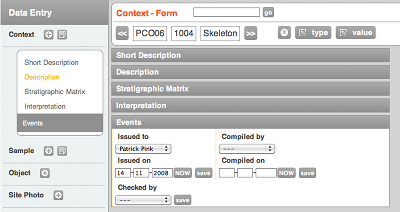
\includegraphics[width=0.8\textwidth]{img/ark_data_entry}
				\label{fig:data_entry}
			\end{figure}
		\end{frame}

		% -----------------------------------------------------

		\begin{frame}{ARK}
		\framesubtitle{Screenshot}
			\begin{figure}
				\centering
				\caption[Vista dei \emph{record} in Ark.]{Vista dei \emph{record} in Ark.}
				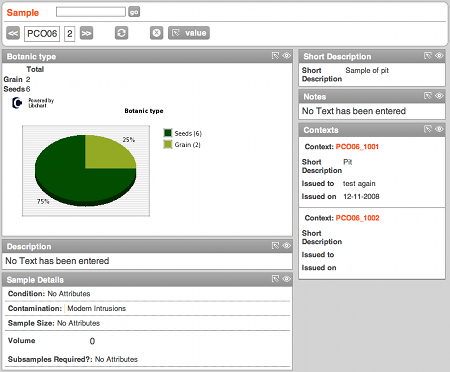
\includegraphics[width=0.7\textwidth]{img/ark_record_view}
				\label{fig:data_entry}
			\end{figure}
		\end{frame}

		% -----------------------------------------------------

		\begin{frame}{ARK}
		\framesubtitle{Screenshot}
			\begin{figure}
				\centering
				\caption[Elenco US/SCR in Ark.]{Elenco US/SCR in Ark.}
				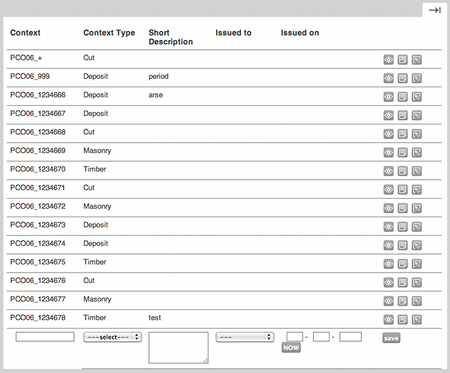
\includegraphics[width=0.7\textwidth]{img/ark_register}
				\label{fig:data_entry}
			\end{figure}
		\end{frame}

		% -----------------------------------------------------

		\begin{frame}{ARK}
		\framesubtitle{Prossimamente\dots}
			Collaborando con L.-P. Archaeology, O.I.A. implementerà:
			\begin{itemize}
				\item esportazione cartografica avanzata con Mapnik
				\item esportazione delle schede di US/SCR in \LaTeX
				\item integrazione modelli 3D in schede \LaTeX~usando MeshLab, U3D e \texttt{movie15}
			\end{itemize}
		\end{frame}

		% -----------------------------------------------------

		\begin{frame}{Grazie!}\label{sli:grazie}
			\begin{center}
				\Huge{Thanks for your time}
				\vfill
				\begin{tikzpicture}[cap=round]
				% Colors
				\colorlet{anglecolor}{green!50!black}
				\colorlet{bordercolor}{black}

				\def\alpha{5} % degree
				\def\layer{5}

				\begin{scope}[scale=1.5]
				\pgfmathsetmacro\sinTriDiff{sin(60-\alpha)}
				\pgfmathsetmacro\cosTriDiff{1-cos(60-\alpha)}
				\pgfmathsetmacro\radiusC{sqrt(\cosTriDiff*\cosTriDiff + \sinTriDiff*\sinTriDiff)}
				\pgfmathsetmacro\startAng{\alpha + atan(\sinTriDiff/\cosTriDiff)}

				\pgfmathsetmacro\al{\alpha*\layer}

				\foreach \x in {0,\alpha,...,\al}
				{
				  \pgfmathsetmacro\ang{\x + \startAng}
				  \pgfmathsetmacro\xRs{\radiusC*cos(\ang)}
				  \pgfmathsetmacro\yRs{\radiusC*sin(\ang)}

				  \pgfmathsetmacro\radiusLayer{\xRs + sqrt( 1 - \yRs*\yRs )}

				  \pgfmathsetmacro\angRs{acos(\yRs)}

				  \pgfmathsetmacro\angRss{acos(\radiusC*sin(\ang-\alpha))}


				  \colorlet{anglecolor}{black!\ang!green}

				  \pgfmathsetmacro\step{2*\alpha - 180}
				  \pgfmathsetmacro\stop{180-2*\alpha}
				  \foreach \y in {-180, \step ,..., \stop}
				  {
				    \pgfmathsetmacro\deltaAng{\y-\x}
				    \filldraw[color=anglecolor,draw=bordercolor] 
					(\y-\x:\radiusLayer)    
						arc (-90+\angRs+\deltaAng : \alpha-90+\angRss+\deltaAng :1) 
						arc (\alpha+90-\angRss+\deltaAng : 2*\alpha+90-\angRs+\deltaAng :1)
						arc (\deltaAng+2*\alpha : \deltaAng : \radiusLayer);
				  }



				}
				\pgfmathsetmacro\xRs{\radiusC*cos(\al+\startAng)}
				\pgfmathsetmacro\yRs{\radiusC*sin(\al+\startAng)}
				\pgfmathsetmacro\radiusLayer{\xRs + sqrt( 1 - \yRs*\yRs )}
				\draw[line width=2, color=bordercolor] (0,0) circle (.8*\radiusLayer);
				\pgfmathsetmacro\radiusSmall{.7*\radiusLayer}
				\foreach \x in {-60,0,...,240}
				{
				    \fill[color=anglecolor] (\x:\radiusSmall) arc (-180+\x+60: -180+\x: \radiusSmall)
							     arc (0+\x: -60+\x: \radiusSmall)
							     arc (120+\x: 60+\x: \radiusSmall); 
				}
				\foreach \x in {0, 4, ..., 360}
				{
				  \fill[color=anglecolor] (\x:1) -- (\x+3:1.05) -- (\x+5:1.05) -- (\x+2:1) -- cycle;
				  \fill[color=anglecolor] (\x+5:1.05) -- (\x+7:1.05) -- (\x+4:1.1) -- (\x+2:1.1) -- cycle;
				}
				\draw[line width=1, color=bordercolor] (0,0) circle (1);
				\draw[line width=1, color=bordercolor] (0,0) circle (1.1);
				\end{scope}

				\end{tikzpicture}
				\vfill
				\huge{and keep Free Software rockin'}
			\end{center}
		\end{frame}

		% -----------------------------------------------------

		\begin{frame}{Credits and licence}
			\begin{center}
				\Huge{\ccbyncsa}
			\end{center}
			\vfill
			\begin{itemize}
				\item ``Mosaic from Pompeii'', Daniel Steger\footnote{\url{www.texample.net/tikz/examples/mosaic-from-pompeii/}.}, in slide \ref{sli:grazie}
				\item Modified version of ``Computer Science Mindmap'', Till Tantau\footnote{\url{www.texample.net/tikz/examples/computer-science-mindmap/}.}, in slide \ref{sli:social}
			\end{itemize}
			\vfill
			
\includegraphics[width=0.1\textwidth]{img/logoreg_1}
			\hfill
			
\includegraphics[width=0.2\textwidth]{img/logoreg_2}
		\end{frame}
\end{document}
